%auto-ignore
\providecommand{\MainFolder}{..}
\documentclass[\MainFolder/Text.tex]{subfiles}


\begin{document}

\section{Hodge propagator} \label{Section:Proof1}

\Correct[inline,caption={DONE Notation for piH}]{We should define the special deformation retract by requiring only $\Htp \iota_\Harm = 0$!! The notation $\Htp \pi_\Harm = 0$ does not make much sense! It makes.}

We will use fiberwise integration and spherical blow-ups, which we now recall.


\begin{Definition}[Fiberwise integration] \label{Def:FibInt}
Let $\Pr: E \rightarrow B$ be a smooth oriented fiber bundle with an oriented fiber $F$ over an oriented manifold~$B$ with $\Bdd B = \emptyset$. We orient $E$ as $F\times B$. Let 
$\DR_{\mathrm{c}} (B)$ denote the space of forms with compact support and $\DR_{\mathrm{cv}}(E)$ the space of forms with compact vertical support. For any $\kappa\in \DR_{\mathrm{cv}}(E)$, let $\FInt{F} \kappa \in \DR(B)$ be the unique smooth form such that
\begin{equation*} \label{Eq:FiberInt}
\int_E \kappa \wedge \Pr^*\eta = \int_B \Bigl(\FInt{F}\kappa \Bigr) \wedge \eta\quad\text{for all }\eta\in \DR_{\mathrm{c}} (B).
\end{equation*}
\end{Definition}
 
\begin{Definition}[Spherical blow-up] Let $X$ be a smooth $n$-dimensional manifold and $Y\subset X$ a smooth $k$-dimensional submanifold. The \emph{blow-up} of $X$ at $Y$ is as a set defined by
$$ \Bl_Y X \coloneqq X\backslash Y \sqcup P^+N Y, $$
where $P^+N Y$ is the real oriented projectivization of the normal bundle $NY$ of~$Y$ in $X$. This means that $P^+NY$ is the quotient of $\{ v\in NY\,
\vert\, v\neq 0\}$ by the relation $v\sim a v$ for all $a\in (0,\infty)$. The \emph{blow-down map} is defined by
\begin{align*}
 \pi : \Bl_Y X &\longrightarrow X \\
     p\in X\backslash Y &\longmapsto p, \\
     [v]_p\in P^+N Y &\longmapsto p.
\end{align*}
\end{Definition}

In the following, we will equip the blow-up with the structure of a smooth manifold with boundary such that its interior becomes diffeomorphic to $X\backslash Y$ via the blow-down map and the boundary becomes $P^+ NY$. Consider an adapted chart $(U,\psi)$ for $Y$ in $X$ with $\psi(U)=\R^{n}$ and $\psi(U\cap Y)=\{(0,y)\mid y\in \R^k \}$. It induces the bijection\Correct[caption={DONE Blow up charts}]{It is not a bijection if $\psi(U\cap Y) \neq \emptyset$! We need it centered at $(0,0)$! No we need actually only the intersection with $Y$!}
\begin{align*}
 \tilde{\psi}: \Bl_{U\cap Y}U &\longrightarrow [0,\infty) \times \Sph{n-k-1} \times \R^k \\
  p\in U\backslash Y &\longmapsto \Bigl (\Abs{\pi_1 \psi(p)}, \frac{\pi_1\psi(p)}{\Abs{\pi_1\psi(p)}},\pi_2 \psi(p) \Bigr), \\
  [v]\in P^+N_p Y & \longmapsto \Bigl(0,\frac{\pi_1 \Diff{\psi}(v)}{\Abs{\pi_1 \Diff{\psi} (v)}},\pi_2\psi(p)\Bigr),
\end{align*}
where $\pi_1$ and $\pi_2$ are the canonical projections to the factors of $\R^{n-k} \times \R^k$. Notice that we have the canonical inclusion $\Bl_{U\cap Y} U \subset \Bl_Y X$. It can be checked that for any two overlapping adapted charts $(U_1,\psi_1)$ and $(U_2,\psi_2)$, the transition function $\tilde{\psi}_1\circ \tilde{\psi}_2^{-1}$ is a diffeomorphism of manifolds with boundary. Therefore, we can use the charts $(\Bl_{U\cap Y}U, \tilde{\psi})$ to define a smooth atlas on~$\Bl_Y X$. If $X$ is oriented, we orient $\Bl_Y X$ so that $\pi$ restricts to an orientation preserving diffeomorphism of the interior.

An important fact is that if $X$ is compact, then \emph{$\Bl_Y X$ is compact}.

We are interested in the case when $X = M\times M$ for an oriented closed manifold $M$ and $Y = \Delta \coloneqq \{(m,m) \mid m\in M\}$ is the \emph{diagonal}. Given a chart $\varphi: U \rightarrow \R^n$ on~$M$, the following is a smooth chart on $\Bl_\Diag(M\times M)$:
\begin{equation} \label{Eq:BlowUpChart}
\begin{aligned}
\tilde{\varphi}: \Bl_{\Diag}(U\times U) & \longrightarrow [0,\infty) \times \Sph{n-1} \times \R^n \\
(x,y)\in (U\times U)\backslash \Diag & \longmapsto  (r,w,u)\coloneqq \begin{multlined}[t] \Bigl(\frac{1}{2}\Abs{\varphi(x)-\varphi(y)}, \frac{\varphi(x)-\varphi(y)}{\Abs{\varphi(x)-\varphi(y)}},\\\frac{1}{2}(\varphi(x)+\varphi(y))\Bigr),\end{multlined} \\
[(v,-v)]_{(x,x)} &\longmapsto \Bigl(0,\frac{\Dd \varphi_x(v)}{\Abs{\Dd \varphi_x(v)}},\varphi(x)\Bigr).
\end{aligned}
\end{equation}
The inverse relations for $r>0$ read
\begin{equation*} \label{Eq:BlowupRelations}
\varphi(x) = u+w r\quad\text{and}\quad\varphi(y)=u-w r.
\end{equation*}
We will denote by $M_i$ the $i$-th factor of $M\times M$; i.e., we will write $M \times M = M_1 \times M_2$. We denote the corresponding projection by $\Pr_i$. We define $\widetilde{\Pr}_i \coloneqq \Pr_i\circ\pi$, where $\pi: \Bl_\Diag(M\times M) \rightarrow M \times M$ is the blow-down map. We also identify $(M\times M)\backslash \Diag$ with the interior of $\Bl_\Diag(M\times M)$ via $\pi$.

\begin{Example}[Product minus open thickening of diagonal]
We have the following examples:
$$\Bl_\Diag(\R\times \R) \simeq \vcenterline{\begin{tikzpicture}
\draw[->] (0,-1) -- (0,2) node[left] {$y$};
\draw[->] (-1,0) -- (2,0) node[below] {$x$};
\draw[thick,red, domain=-.8:1.6] plot (\x, {\x + .2});
\foreach \i in {0,...,20}
{\draw[dotted,gray] ($({2.4/20*\i - .8},1.8)$) -- ($({2.4/20*\i - .8},{2.4/20*\i - .8+ .2})$);
}
\draw[thick,red, domain=-.8:1.8] plot (\x, {\x - .2});
\foreach \i in {0,...,20}
{\draw[dotted,gray] ($({2.6/20*\i - .8},-1)$) -- ($({2.6/20*\i - .8},{2.6/20*\i - .8 - .2})$);
}
\end{tikzpicture}}
\qquad
\Bl_\Diag(\Sph{1}\times \Sph{1}) \simeq 
\vcenterline{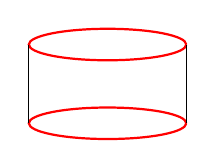
\begin{tikzpicture}
\draw[thick,red] (0,1) arc (0:360:{1} and {.2});
\draw[thick,red] (0,0) arc (0:360:{1} and {.2});
\draw (0,0) -- (0,1);
\draw (-2,0) -- (-2,1);
\end{tikzpicture}}$$
In fact, the manifold $\Bl_\Diag(M\times M)$ is always diffeomorphic to $M\times M$ minus an open thickening of the diagonal. The blow-down map is therefore an essential part of the blow-up construction.
\end{Example}


The map $\widetilde{\Pr}_2: \Bl_\Diag(M\times M) \rightarrow M_2$ is an oriented fiber bundle with fiber $\Bl_{*}(M_1)$, which is the blow-up of $M_1$ at a point (we shall assume that $M$ is connected). The \emph{fiberwise integration along~$\widetilde{\Pr}_2$} will be denoted by~$\FInt{\Bl_* M_1}$. 

\begin{Def}[Hodge propagator] \label{Def:GreenKernel}
Let $M$ be an oriented closed $n$-dimensional Riemannian manifold. Consider the harmonic projection $\pi_{\Harm}$ from \eqref{Eq:HarmProj}, and let $\iota_{\Harm}: \Harm(M) \xhookrightarrow{} \DR(M)$ be the inclusion. 
A smooth $(n-1)$-form $\Prpg$ on $(M\times M)\backslash \Diag$ is called an \emph{admissible Hodge propagator} if the following conditions are satisfied:
\begin{PlainList}
\item The form $\Prpg$ admits a smooth extension to $\Bl_\Diag(M\times M)$. More precisely, the pullback $(\Restr{\pi}{\mathrm{int}})^* \Prpg$ along the blow-down map restricted to the interior is a restriction of a smooth form on $\Bl_\Diag(M\times M)$. We denote this form by $\Prpg$ again by uniqueness.
%We can denote this form by~$\Prpg$ again by uniqueness of the extension.
\item The operator $\Htp: \DR^*(M) \rightarrow \DR^{*-1}(M)$ defined by
\begin{equation} \label{Eq:SchwKer}
\Htp(\eta) \coloneqq \FInt{\Bl_* M_1} \Prpg \wedge \widetilde{\Pr}_1^* \eta \quad \text{for all }\eta\in \DR(M)
\end{equation}
satisfies
%\marginnote{What definition of the Hodge propagator do I actually need?}
\begin{equation} \label{Eq:CochainHomotopy}
\Dd\circ\Htp + \Htp\circ\,\Dd = \iota_{\Harm}\circ \pi_{\Harm} - \Id.
\end{equation}
Any homogenous linear operator $\Htp: \DR^*(M) \rightarrow \DR^{*-1}(M)$ satisfying~\eqref{Eq:CochainHomotopy} will be called a \emph{Hodge homotopy}.% We sometimes refer to $\Prpg$ as the Schwartz kernel of $\Htp$.
\item For the twist map $\tau: M \times M \rightarrow M \times M$ defined by $(x,y)\mapsto (y,x)$, the following symmetry property holds:
\begin{equation}\label{Eq:SymProp}
\tau^* \Prpg = (-1)^n \Prpg. 
\end{equation}
\end{PlainList}
\end{Def}

\begin{Remark}[On Hodge propagator]\phantomsection\label{Rem:GKer}
\begin{RemarkList}
\item Given a homogenous linear operator $\Htp: \DR^*(M) \rightarrow \DR^{*-1}(M)$, if there is a $\Prpg \in \DR^{n-1}(\Bl_{\Diag}(M\times M))$ such that \eqref{Eq:SchwKer} holds, then it is unique.
\item Because $\tau: M\times M \rightarrow M\times M$ preserves $\Diag$, it extends to a diffeomorphism $\tilde{\tau}$ of $\Bl_\Diag(M\times M)$. The condition \eqref{Eq:SymProp} is then equivalent to $\tilde{\tau}^*\tilde{\Prpg} = (-1)^n \tilde{\Prpg}$ for the extension $\tilde{\Prpg}$ of $\Prpg$ to $\Bl_{\Diag}(M\times M)$. We denote both extensions by $\tau$ and $\Prpg$, respectively.

\item Using the intersection pairing $(\cdot,\cdot)$, we have 
$$ \begin{aligned}(\Htp(\eta_1),\eta_2) &= \int_{\Bl_{\Diag}(M\times M)} \Prpg \wedge \widetilde{\Pr}_1^*\eta_1 \wedge \widetilde{\Pr}_2^*\eta_2 \\ 
&= (-1)^n \int_{\Bl_{\Diag}(M\times M)} \tau^*\Prpg \wedge \widetilde{\Pr}_2^*\eta_1 \wedge \widetilde{\Pr}_1^*\eta_2 \end{aligned}$$
and 
$$ \begin{aligned}(\eta_1, \Htp(\eta_2)) &= (-1)^{\eta_1(\eta_2 - 1)} (\Htp(\eta_2),\eta_1) \\ &= (-1)^{\eta_1} \int_{\Bl_\Diag(M\times M)} \Prpg \wedge \widetilde{\Pr}_2^* \eta_1 \wedge \widetilde{\Pr}_1^* \eta_2 \end{aligned}$$
for all $\eta_1$, $\eta_2\in \DR(M)$. This implies the following:
\begin{equation}\label{Eq:GSA}
\tau^* \Prpg = (-1)^n \Prpg \quad \Longleftrightarrow \quad \begin{multlined}[t](\Htp(\eta_1),\eta_2) = (-1)^{\eta_1}(\eta_1, \Htp(\eta_2)) \\ \forall \eta_1, \eta_2 \in\DR(M). \end{multlined}
\end{equation}

\item Because $\Bl_\Diag(M\times M)$ is compact, $\Prpg\in \DR(\Bl_\Diag(M\times M))$ induces an $L^1$-integrable form on $M\times M$.

\item In the original article \cite{Cieliebak2015}, Hodge propagator is called ``Green kernel''. However, this term is standardly used to denote the Schwartz kernel of the generalized inverse of an elliptic pseudo-differential operator, e.g., of the Laplacian $\Delta$. Because this caused confusion in discussions, we decided to change it to Hodge propagator. This turned out to appear already in \cite{Cattaneo2015}. This is how we discovered \cite{Mnev2009}, where this problematic was also treated, and where we took the trick in the proof of Proposition~\ref{Prop:ExistenceG} from.
\qedhere
\end{RemarkList}
\end{Remark}

We will now prove three propositions which will allow us to rewrite~\eqref{Eq:CochainHomotopy} equivalently as a differential equation for $\Prpg$ on $M\times M \backslash \Diag$.


\begin{Proposition}[Identities for fiberwise integration]\label{Prop:StokesForm}
In the situation of Definition~\ref{Def:FibInt},
assume that $F$ has a boundary $\Bdd F$. We orient $\Bdd F$ using $T_p F = N(p)\oplus T_p \Bdd F$ for $p\in \Bdd F$, where $N$ is an outward pointing normal vector field.
The following formulas hold for all $\kappa\in \DR_{\mathrm{cv}}(E)$ and $\eta\in \DR_{\mathrm{c}}(B)$:
\begin{itemize}
\item The \emph{projection formula}
$$\FInt{F}(\kappa\wedge \pi^* \eta) = \Bigl(\FInt{F}\kappa\Bigr)\wedge \eta, $$
\item \emph{Stokes' formula}
$$(-1)^F \Dd \FInt{F}\kappa  = \FInt{F} \Dd \kappa -  \FInt{\Bdd F} \kappa, $$
where $F$ in the exponent denotes the dimension of $F$.
\end{itemize}
\end{Proposition} 
%
\begin{proof} % Checked on 23.9.17
The projection formula is proven by a straightforward calculation from the definition.

As for Stokes' formula, we get the oriented fiber bundle $\Bdd E \rightarrow B$ with fiber~$\Bdd F$ by restricting an oriented trivialization of $E$. There are two orientations on $\Bdd E$ --- as the total space of $\Bdd E \rightarrow B$ and as the boundary of $E$. They agree due to our orientation convention. Using standard Stokes' theorem, we get
\allowdisplaybreaks
\begin{align*}
 (-1)^F \int_B \Dd \Bigl(\FInt{F}\kappa\Bigr) \wedge \eta & = (-1)^{\kappa + 1} \int_B \Bigl(\FInt{F}\kappa\Bigr)\wedge \Dd \eta \\ &=  (-1)^{\kappa + 1} \int_{E} \kappa \wedge \Dd \pi^*\eta \\
  & = \int_E \bigl(\Dd \kappa \wedge \pi^*\eta - \Dd(\kappa \wedge\pi^*\eta)\bigr) \\ 
  &= \int_B \Bigl(\FInt{F} \Dd \kappa\Bigr) \wedge \eta - \int_{\Bdd E} \kappa \wedge \pi^*\eta \\ 
  &= \int_B \Bigl(\FInt{F} \Dd \kappa - \FInt{\Bdd F}\kappa \Bigr) \wedge \eta.
\end{align*}
This proves the proposition.
\end{proof}

In what comes next, we will view the canonical projection $\Pr_2 : M_1 \times M_2 \rightarrow M_2$ as an oriented fiber bundle such that the orientation of the total space agrees with the product orientation. The fiberwise integration for this bundle will be denoted by $\FInt{M_1}$. 

\begin{Proposition}[Schwartz kernel of the harmonic projection] \label{Lemma:HKer}
Let $M$ be an oriented closed $n$-dimensional Riemannian manifold. Let $\Le_1$,~$\dotsc$, $\Le_m$ be a homogenous basis of $\Harm(M)$ which is orthonormal with respect to the $L^2$-inner product 
$$ (\eta_1, \eta_2)_{L^2} \coloneqq \int_M \eta_1 \wedge \Star\eta_2\quad\text{for }\eta_1, \eta_2 \in \DR(M), $$
where $\Star$ denotes the Hodge star. The smooth form $\HKer \in \DR^n(M\times M)$ defined by
\begin{equation}\label{Eq:HKerHKerHKer}
\HKer \coloneqq \sum_{i=1}^m (-1)^{n \Le_i}\Pr_1^*(\Star \Le_i) \wedge \Pr_2^*(\Le_i)
\end{equation}
satisfies the following properties:
\begin{ClaimList}
\item For all $\eta\in \DR(M)$, we have
\begin{equation*}
 \HPr(\eta) = \FInt{M_1} \HKer\wedge \Pr_1^*\eta.
\end{equation*} 
\item The form $\HKer$ is closed and Poincar\'e dual to $\Diag \subset M\times M$.
\item The following symmetry condition is satisfied:
\begin{equation} \label{Eq:SymHKer}
\tau^* \HKer = (-1)^n \HKer.
\end{equation}
\end{ClaimList}
\end{Proposition}
%
\begin{proof} % Checked on 25.9.17
\begin{ProofList}
\item For the purpose of the proof, we denote $\Harm(\eta) \coloneqq \FInt{M_1} \HKer \wedge \Pr_1^* \eta$. For every $k=1$,~$\dotsc$, $m$, we use the projection formula to compute
%
\allowdisplaybreaks
\begin{align*}
\Harm(\Le_k) &= \sum_{i=1}^m (-1)^{\Le_i n+\Le_i \Le_k}\FInt{M_1} \Pr_1^*(\Star \Le_i \wedge \Le_k)\wedge \Pr_2^*(\Le_i) \\ &=\sum_{i=1}^m (-1)^{\Le_i(n+\Le_k) + \Le_k(n+\Le_i)}\Bigl(\int_M \Le_k \wedge \Star \Le_i\Bigr) \Le_i \\
 & = \Le_k.
\end{align*}
It is easy to see that $\Harm(\eta) \in \Harm(M)$ for all $\eta\in \DR(M)$. Therefore, $\Harm$ is a projection to $\Harm(M)$. Relations $\Harm(\Dd \eta) = \Harm(\CoDd \eta) = 0$ for all $\eta\in \DR(M)$ follow from the second line of the computation above with $\Le_k$ replaced by $\Dd\eta$ and $\CoDd\eta$ using that $\Im \CoDd \oplus \Im \Dd$ is $L^2$-orthogonal to $\Harm(M)$. We see that $\Harm = \pi_{\Harm}$. 

\item Using $\Dd \circ \Harm = \Harm \circ \Dd = 0$ and Stokes' theorem, we get 
$$  \FInt{M_1} \Dd \HKer \wedge \Pr_1^* \eta = (-1)^n \Dd \Harm(\eta) - \Harm(\Dd \eta) = 0\quad \text{for all }\eta\in \DR(M). $$
It follows that $\Dd \HKer = 0$. Using the K\"unneth formula, we can write a given $\kappa\in \DR(M\times M)$ with $\Dd \kappa = 0$ as $\kappa = \Pr_1^* \eta_1 \wedge \Pr_2^* \eta_2 + \Dd \eta$ for some $\eta_1$, $\eta_2 \in \Harm(M)$ and $\eta\in \DR(M)$. Then 
$$ \begin{aligned} \int_{M\times M} \HKer \wedge \kappa & = \int_{M\times M} \HKer \wedge \Pr_1^* \eta_1 \wedge \Pr_2^* \eta_2 \\ &= \int_M \Harm(\eta_1)\wedge \eta_2 \\ &= \int_M \eta_1 \wedge \eta_2 = \int_{\Diag} \kappa. \end{aligned} $$
This shows that $\HKer$ is Poincar\'e dual to $\Diag$.
\item It follows from the Hodge decomposition that
\begin{equation}\label{Eq:HKerHKer}
(\pi_\Harm(\eta_1), \eta_2) = (\pi_{\Harm}(\eta_1), \pi_{\Harm}(\eta_2)) = (\eta_1,\pi_\Harm(\eta_2))\quad\text{for all }\eta_1, \eta_2 \in \DR(M).
\end{equation}
As in (iii) of Remark \ref{Rem:GKer}, one shows that this is equivalent to \eqref{Eq:SymHKer}.\qedhere
\end{ProofList}
\end{proof}



\begin{Proposition}[Differential condition] \label{Prop:GKer}
Let $M$ be an oriented closed $n$-dimensional Riemannian manifold. For $\Prpg \in \DR^{n-1} (\Bl_\Delta(M\times M))$,  the following claims are equivalent:
\begin{PlainList} 
\item The operator $\Htp: \DR^*(M) \rightarrow \DR^{*-1}(M)$ defined by $\Htp(\eta) \coloneqq \FInt{\Bl_* M_1} \Prpg \wedge \widetilde{\Pr}_1^*\eta$ for $\eta\in \DR(M)$ is a Hodge homotopy.
%, i.e.~Equation~\eqref{Eq:CochainHomotopy} from Definition~\ref{Def:GreenKernel} holds.
\item It holds \begin{equation} \label{Eq:GKer}
 \Dd \Prpg = (-1)^{n} \HKer\quad\text{on }(M\times M)\backslash \Delta.
\end{equation} 
\end{PlainList}
\end{Proposition}
%
\begin{proof} % Checked on 26.9.17 
Before we begin, note that~\eqref{Eq:GKer} is equivalent to the equation $\Dd \tilde{\Prpg} = (-1)^n \pi^* \HKer$ on $\Bl_\Diag(M\times M)$ for the extension $\tilde{\Prpg}$ of $\Prpg$; we denote~$\tilde{\Prpg}$ by~$\Prpg$ and $\pi^*\HKer$ by $\HKer$ by uniqueness.

We will first prove $2) \Longrightarrow 1)$.
%By uniqueness of smooth extension to the boundary we have
%$$ \Dd \Prpg = (-1)^{n}\pi^* H $$
%on $\Bl_\Diag(M\times M)$.
Using Stokes' formula, we get for every $\eta\in \DR(M)$ the following:
%
\begin{equation*}
\begin{aligned}
  \Dd \Htp (\eta) &= \Dd \FInt{\Bl_* M_1} \Prpg\wedge \widetilde{\Pr}_1^* \eta \\ 
  &= (-1)^n \Bigl( \FInt{\Bl_* M_1} \Dd(\Prpg\wedge\widetilde{\Pr}_1^* \eta) - \FInt{\Bdd \Bl_* M_1} \Prpg \wedge \widetilde{\Pr}_1^* \eta \Bigr) \\ 
  &= \HPr(\eta) - \Htp(\Dd\eta) +  \FInt{\Bdd \Bl_* M_1} (-1)^{n+1}\Prpg\wedge \widetilde{\Pr}_1^*\eta.
\end{aligned}
\end{equation*}
Since $\widetilde{\Pr}_1 = \widetilde{\Pr}_2$ on $\Bdd \Bl_\Diag (M\times M)$, we get with the help of the projection formula the following:
\begin{equation*}
 \FInt{\Bdd \Bl_* M_1} \Prpg\wedge \widetilde{\Pr}_1^*\eta  = \FInt{\Bdd \Bl_* M_1} \Prpg\wedge \widetilde{\Pr}_2^*\eta = \Bigl(\FInt{\Bdd \Bl_* M_1} \Prpg \Bigr)\wedge\eta.
\end{equation*}
We will show that the $0$-form $\FInt{\Bdd \Bl_* M_1} \Prpg$ is constant $(-1)^n$. Stokes' formula implies
\begin{equation*}
 \FInt{\Bdd \Bl_* M_1} \Prpg = \FInt{\Bl_* M_1} \Dd \Prpg = (-1)^n \FInt{\Bl_* M_1} \HKer. 
\end{equation*}
Using that $\HKer$ is Poincar\'e dual to $\Diag$, we get for every $\eta\in \DR^n(M)$ the following:
%
\begin{equation*}
\begin{aligned}
 \int_M \Bigl(\FInt{\Bl_* M_1} \HKer \Bigr) \wedge \eta &= \int_{\Bl_\Diag(M\times M)} \HKer\wedge \widetilde{\Pr}_2^*\eta 
 \\ &= \int_{M\times M} H\wedge \Pr_2^*\eta  \\ &= \int_\Diag \Pr_2^*\eta  = \int_M 1\wedge \eta.
\end{aligned}
\end{equation*}
The implication follows.

We will now prove $1) \Longrightarrow 2)$. Assume that~\eqref{Eq:CochainHomotopy} holds and that~$\Prpg$ extends smoothly to the blow-up. Denote
$$K\coloneqq (-1)^n \Dd \Prpg - \HKer\quad\text{and}\quad L\coloneqq -1 +  \int^{\Bdd \Bl_*(M_1)} (-1)^n \Prpg. $$
Notice that $L$ is a function on $M$. From the previous computations, we deduce that 
$$ \int^{\Bl_*(M_1)} K\wedge \widetilde{\Pr}_1^*\eta = L\eta\quad\text{for all }\eta\in \DR(M), $$
and hence
$$ \int_{\Bl_{\Diag}(M\times M)} K \wedge \widetilde{\Pr}_1^*(\eta_1) \wedge \widetilde{\Pr}_2^*(\eta_2)  = \int_M L \eta_1 \wedge \eta_2 \quad\text{for all }\eta_1, \eta_2 \in \DR(M). $$
If $K(x,y) \neq 0$ for some $(x,y)\in (M\times M)\backslash\Delta$, we can choose $\eta_1$, $\eta_2$ with disjoint supports such that the left-hand side is non-zero. This is a contradiction. Consequently, we have $K\equiv 0$.
\end{proof}

In general, the \emph{Schwartz kernel} of a linear operator $\Htp: \DR(M) \rightarrow \DR(M)$ is a distributional form $\Prpg$ on $M\times M$ which satisfies\footnote{We may consider such class of $\Htp$'s, e.g., pseudo-differential operators, such that $\Prpg$ exists and is unique (c.f., the well-known Schwartz kernel theorem).} 
\begin{equation*} 
\Htp(\eta)(x) = \int_{y\in M_1} \Prpg(y,x)\eta(y)\quad\text{for all }\eta\in \DR(M)\text{ and }x\in M_2.
\end{equation*}
We consider the following conditions on $\Htp$ and $\Prpg$:\label{ConditionsG}\Correct[caption={Typo},disable]{There is ''of'' missing downstairs.} 
\begin{center}
\begin{minipage}{.9\textwidth}
\begin{enumerate}[label=(G\arabic*)]
\item The Schwartz kernel $\Prpg$ of $\Htp$ is a restriction of a smooth form on $\Bl_\Diag(M\times M)$.
\item $\Dd\circ \Htp + \Htp\circ \Dd = \iota_{\Harm} \circ \pi_\Harm - \Id$.
\item $(\Htp(\eta_1),\eta_2) = (-1)^{\eta_1}(\eta_1,\Htp(\eta_2))$ for all $\eta_1$, $\eta_2\in \DR(M)$.
\item $\Htp \circ \iota_\Harm = 0$, $\pi_\Harm \circ \Htp = 0$.
\item $\Htp \circ \Htp = 0$.
\end{enumerate}
\end{minipage}
\end{center}
Clearly, (P1)--(P3) are equivalent to $\Prpg$ being a Hodge propagator from Definition~\ref{Def:GreenKernel}. Conditions (P4) and (P5) play a crucial role in the vanishing results for the Chern-Simons Maurer-Cartan element $\PMC$ in Section~\ref{Sec:Vanishing} --- the more conditions are satisfied, the more vanishing we get.

The following lemma will be used in the proof of the upcoming proposition.
\begin{Lemma}\label{Lem:Smoothing}
Let $\Htp_1$, $\Htp_2$ be two linear operators $\DR(M) \rightarrow \DR(M)$ with Schwartz kernels $\Prpg_1$, $\Prpg_2 \in \DR(\Bl_\Diag(M\times M))$. Then $\Htp\coloneqq \Htp_1 \circ \Htp_2$ is a smoothing operator, i.e., its Schwartz kernel $\Prpg$ is a smooth form on $M\times M$. 
\end{Lemma}
\begin{proof}
It holds $\Prpg(x_1,x_2) = \pm \int_x \Prpg_2(x_1,x) \Prpg_1(x,x_2)$. The lemma follows from properties of convolution.
\end{proof}

A version of the following proposition can be found in \cite{Mnev2009}.
\begin{Proposition}[Existence of special Hodge propagator] \label{Prop:ExistenceG}
Every oriented closed Riemannian manifold $M$ admits a special Hodge propagator.
%Moreover, we can choose it such that the corresponding Green operator $\Htp$ satisfies
%\begin{equation} \label{Eq:SpecialProp}
%\Htp \circ \pi_{\Harm} = \pi_\Harm \circ \Htp = 0.
%\end{equation}
\end{Proposition}

\begin{proof}[Proof of Proposition \ref{Prop:ExistenceG}]
Because $\HKer$ is Poincar\'e dual to $\Diag$, we have for any closed $\kappa \in \DR_{\mathrm{c}}((M\times M)\backslash \Delta)$ the following:
$$ \int_{(M\times M)\backslash \Diag} \HKer \wedge \kappa = \int_{M\times M} \HKer \wedge \kappa = \int_{\Diag} \kappa = 0. $$
Poincar\'e duality for non-compact oriented manifolds (see \cite{BottTu1982}) implies that $\HKer$ is exact on $(M\times M)\backslash \Diag$. Because a manifold with boundary is homotopy equivalent to its interior,  the restriction of the blow-down map induces an isomorphism $\pi^* : \HDR((M\times M)\backslash \Diag) \rightarrow \HDR(\Bl_{\Diag}(M\times M))$. It follows that $(-1)^n \pi^* \HKer$ admits a primitive $\Prpg \in \DR(\Bl_{\Diag}(M\times M))$. According to Proposition~\ref{Prop:GKer}, the corresponding $\Htp$ satisfies (P1) and (P2).

If we define
$$ \tilde{\Prpg} \coloneqq \frac{1}{2}(\Prpg + (-1)^n \tau^* \Prpg)\in \DR^{n-1}(\Bl_{\Diag}(M\times M)), $$
then $\tilde{\Prpg}$ satisfies $\tau^* \tilde{\Prpg} = (-1)^n \tilde{\Prpg}$ and is still a primitive to $(-1)^n \pi^* \HKer$. Proposition~\ref{Prop:GKer} and \eqref{Eq:GSA} imply that the corresponding $\Htp$ satisfies (P1)--(P3).

Given $\Htp$ satisfying (P1)--(P3), we will now show that we can arrange (P4). Let us define
$$ \tilde{\Htp}\coloneqq (\Id - \pi_{\Harm}) \circ \Htp \circ (\Id - \pi_{\Harm}), $$
where we view $\pi_{\Harm}$ as a map $\pi_{\Harm}: \DR \rightarrow \Harm \subset \DR$. Then $\tilde{\Htp}$ is a Hodge homotopy because
$$ \Dd\circ\tilde{\Htp} + \tilde{\Htp} \circ \Dd = (\Id-\pi_{\Harm})\circ (\Dd\circ \Htp + \Htp \circ \Dd) \circ (\Id-\pi_{\Harm}) = \Id-\pi_{\Harm}. $$
Using \eqref{Eq:HKerHKer} and \eqref{Eq:GSA}, we see that $\tilde{\Htp}$ satisfies (P3). Using the intersection pairing and Proposition~\ref{Lemma:HKer}, we can write 
$$ \pi_{\Harm}(\eta) = \sum_{i=1}^m (-1)^{(n+\eta)\Le_i} (\Star \Le_i, \eta) \Le_i \quad\text{for all }\eta\in\DR(M),$$
and hence we have for all $\eta_1$, $\eta_2\in \DR(M)$ the following:
$$ \begin{aligned}
&\bigl(\Htp(\pi_{\Harm}(\eta_1)),\eta_2\bigr) = \sum_{i=1}^m (-1)^{(n+\eta_1)\Le_i} (\Star \Le_i, \eta_1) \bigl(\Htp(\Le_i), \eta_2\bigr) \\ 
& \qquad = \sum_{i=1}^m (-1)^{(n+1)\Le_i}  \int_{M\times M}\Pr_1^*(\Star \Le_i)\wedge \Pr_2^*(\Htp(\Le_i))\wedge \Pr_1^*(\eta_1)\wedge \Pr_2^*(\eta_2).
\end{aligned} $$
It follows that the Schwartz kernel of $\Htp \circ \pi_{\Harm}$ is the smooth form
$$ \Kern_{\Htp\circ \pi_{\Harm}} \coloneqq \sum_{i=1}^m (-1)^{(n+1)\Le_i}\Pr_1^*(\Star \Le_i)\wedge \Pr_2^*(\Htp(\Le_i)). $$
Moreover, if we replace $\Htp$ with 
$\pi_{\Harm}\circ \Htp$, we get the smooth Schwartz kernel $\Kern_{\pi_{\Harm}\circ\Htp\circ \pi_{\Harm}}$ of $(\pi_{\Harm}\circ \Htp) \circ \pi_{\Harm}$. In the same way, but now using in addition \eqref{Eq:GSA}, we can write
\allowdisplaybreaks
\begin{align*}
&\bigl(\pi_{\Harm}(\Htp(\eta_1)),\eta_2 \bigr) = (-1)^{\eta_1}\bigl( \eta_1, \Htp(\pi_{\Harm}(\eta_2))\bigr) = (-1)^{\eta_1 \eta_2} \bigl(\Htp(\pi_{\Harm}(\eta_2)),\eta_1\bigr) \\
 &\qquad = \sum_{i=1}^m (-1)^{\eta_1 \eta_2 + (n+1)\Le_i} \int_{M\times M}\Pr_1^*(\Star \Le_i)\wedge \Pr_2^*(\Htp(\Le_i))\wedge \Pr_1^*(\eta_2)\wedge \Pr_2^*(\eta_1) \\
 &\qquad = \sum_{i=1}^m (-1)^{(n+1) \Le_i + n} \int_{M \times M} \Pr_2^*(\Star \Le_i) \wedge \Pr_1^*(\Htp(\Le_i))\wedge \Pr_1^*(\eta_1)\wedge\Pr_2^*(\eta_2),
\end{align*}
where in the last equality we pulled back the integral along the twist map. It follows that the Schwartz kernel of $\pi_{\Harm}\circ \Htp$ is the smooth form
$$ \Kern_{\pi_{\Harm}\circ\Htp} \coloneqq \sum_{i=1}^m (-1)^{\Le_i}\Pr_1^*(\Htp(\Le_i))\wedge \Pr_2^*(\Star \Le_i). $$
The Schwartz kernel of $\tilde{\Htp} = \Htp - \pi_{\Harm}\circ \Htp - \Htp \circ \pi_{\Harm} + \pi_{\Harm}\circ\Htp\circ\pi_{\Harm}$ is then
$$ \tilde{\Prpg} = \Prpg - \pi^* \Kern_{\Htp \circ \pi_{\Harm}} - \pi^* \Kern_{\pi_{\Harm}\circ\Htp} + \pi^* \Kern_{\pi_{\Harm}\circ\Htp\circ\pi_{\Harm}}, $$
which is a smooth form on $\Bl_{\Diag}(M\times M)$. Therefore, $\tilde{\Prpg}$ satisfies (P1)--(P4).

Given $\Htp$ satisfying (P1)--(P4), we will show that we can arrange (P5). The trick from \cite{Mnev2009} is to define
$$ \tilde{\Htp} = \Htp \Dd \Htp. $$
Applying (P1) and (P2) repeatedly, we compute
\begin{equation}\label{Eq:ExprGreen}
\begin{aligned}
\Dd \Htp \Htp \Htp \Dd &= \Dd \Htp \Htp - \Dd \Htp \Htp \Dd \Htp = \Dd \Htp \Htp - \Dd \Htp \Htp + \Dd \Htp \Dd \Htp \Htp \\ &= \Dd \Htp \Htp - \Dd \Dd \Htp \Htp \Htp = \Dd \Htp \Htp = \Htp - \Htp \Dd \Htp, 
\end{aligned}
\end{equation}
and hence
$$ \tilde{\Htp} = \Htp - \Dd \Htp \Htp \Htp \Dd. $$
Clearly, $\tilde{\Htp}$ satisfies (P1) and (P2). As for (P3), we compute
$$ (\eta_1, \tilde{\Htp} \eta_2) = (-1)^{\eta_1}(\Htp \eta_1, \Dd \Htp \eta_2) = (\Dd \Htp \eta_1, \Htp \eta_2) = (-1)^{\eta_1}(\tilde{\Htp}\eta_1,\eta_2). $$
As for (P5), we have
\begin{equation}\label{Eq:GSquared}
\begin{aligned}
\tilde{\Htp} \tilde{\Htp} &= \Htp \Dd \Htp (\Htp\Dd) \Htp = \Htp \Dd \Htp \Htp - \Htp \Dd (\Htp \Dd) \Htp \Htp \\
&= \Htp \Dd \Htp \Htp - \Htp \Dd \Htp \Htp + \Htp \Dd \Dd \Htp \Htp = 0.
\end{aligned}
\end{equation}
In order to show (P4), we have to compute the Schwartz kernel of $\Dd\Htp\Htp\Htp\Dd$. By Lemma \ref{Lem:Smoothing}, the Schwartz kernel $\TKer$ of $\TOp\coloneqq \Htp \Htp \Htp$ is a smooth form on $M \times M$. Therefore, Stokes' formula without the boundary term applies, and we get 
$$ (\Dd \TOp \Dd)\eta = \Dd \int^{M_1} \TKer \wedge \Dd \pi_1^*(\eta) = \int^{M_1} \Dd \TKer \wedge \Dd \pi_1^*(\eta) = (-1)^{\TKer} \int^{M_1} \Dd_1 \Dd \TKer \wedge \pi_1^*(\eta). $$
Here $\Dd_1: \DR(M\times M) \rightarrow \DR(M\times M)$ is the operator defined in local coordinates by
$$ \Dd_1\bigl(f(x,y)\Diff{x}^I\Diff{y}^J\bigr) = \sum_{i=1}^n \frac{\partial f}{\partial x^i}(x,y)\Diff{x^i}\Diff{x}^I \Diff{y}^J. $$
It follows that the Schwartz kernel $\tilde{\Prpg}$ of $\tilde{\Htp}$ satisfies 
$$ \tilde{\Prpg} = \Prpg + (-1)^{n} \Dd_1 \Dd \TKer $$
and is a smooth $(n-1)$-form on $\Bl_\Diag(M\times M)$. Conditions (P1)--(P5) are satisfied. \qedhere
\end{proof}

\begin{Remark}[Property (P5) in dimensions $1$ and $2$]
In dimension $1$, every operator of degree $-1$ satisfies (P5) from degree reasons. In dimension $2$, every operator satisfying (P1) and (P2) satisfies (P5) as well, which follows from \eqref{Eq:ExprGreen} and \eqref{Eq:GSquared}.
\end{Remark}


\begin{Remark}[The standard Hodge propagator]
Consider the Hodge-de Rham Laplacian $\Delta = \Dd \circ \CoDd + \CoDd \circ \Dd : \DR(M) \rightarrow \DR(M)$ and its ``Green operator'' $\GOp$ of degree~$0$ (see (v) of Remark \ref{Rem:GKer} for the collision of terminology) which was defined in~\cite[Definition~6.9]{Warner1983} by
$$\GOp \coloneqq (\Restr{\Delta}{\Harm(M)^{\perp}})^{-1} \circ \pi_{\Harm(M)^\perp}, $$
where $\perp$ denotes the $L^2$-orthogonal complement. We introduce the \emph{standard Hodge homotopy} by
\begin{equation}\label{Eq:GStdStd}
\HtpStd \coloneqq -\CoDd\circ \Htp_{\Delta}.
\end{equation}
Using the properties of $\GOp$, $\Dd$ and $\CoDd$, one can show that $\HtpStd$ satisfies (P2)--(P5).

As for (P1), the author was able to show it for flat manifolds ($\coloneqq$\,locally isometric to $\R^n$) by transforming the following formula inspired by \cite{Harris2004} to blow-up coordinates and explicitly computing the integral and limit:
$$ \PrpgStd = - \lim_{t\to 0} \int_t^\infty \frac{1}{2}\CoDd K_\tau \Diff{\tau}, $$
where $\KKer_t(x,y) = \sum_i (-1)^{n e_i} e^{-\lambda_i t} (\Star e_i)(x) \wedge e_i(y)$ is the heat kernel of $\Delta$ and~$e_i$ the $L^2$-orthonormal eigenbasis of $\Delta$ with eigenvalues $\lambda_i$ (the signs come from our convention for fiberwise integration, c.f., \eqref{Eq:HKerHKerHKer}).
%
%More thoughts about Conj.~\ref{Conj:GStd} using the asymptotic expansion of the heat kernel or the techniques of pseudo-differential operators may appear in~\cite{MyPhD}.
\end{Remark}
\end{document}
